\chapter{Implementasi Dan Pengujian Aplikasi}
\label{chap:implementasi dan pengujian aplikasi}

Pada bab 5 akan dibahas implementasi dan pengujian aplikasi pembuatan \textit{Twitter Bot} untuk mencari jalur transportasi publik.

\section{Lingkungan Pembangunan}
Lingkungan perangkat lunak dan perangkat keras yang digunakan untuk membangun dan menguji aplikasi pembuatan \textit{Twitter Bot} untuk mencari jalur transportasi publik ini adalah:
\begin{itemize}
	\item Komputer
	
	
	\begin{itemize}
		\item Processor: Intel Core i7-2630QM CPU 2.00 GHz
		\item RAM: 4096MB
		\item Hardisk: 211GB
		\item VGA : NVDIA GeForce GT 540M
	\end{itemize}
	\item Sistem operasi: Windows 7 Professional
	\item Platform: NetBeans: IDE 8.0.2
	
	\item Akun Twitter Bot
	\begin{itemize}
		\item Nama akun: kviniink
		\item ConsumerKey : 3iT8duMItTTrdaU1qTHxwDIUl
		\item ConsumerSecret : YUIgJTbQT3i5tYA5RE0L38dPT9HaDhuBTifvVmKDYeOgJ*****
		\item AccessToken : 313287708-NO5SPbreQvoOxtXUD5EcKlubIfCBNfCb6aRqYBlZ
		\item AccessTokenSecret : LVfDgtlfeht5yjBJGSgvSvtMYcFMoEdYOspYoOpt*****
	\end{itemize}
	
	\item Akun Twitter penguji : kviniinktest123
\end{itemize}

\iffalse
\section{Hasil Tampilan Antarmuka}
Pada aplikasi pembuatan \textit{Twitter Bot} untuk mencari jalur transportasi publik ini memiliki tampilan antarmuka berbasis teks yang berguna untuk melihat hasil penangkapan tweet, dan hasil tweet yang diberikan kepada user. Sedangkan user dapat mencoba aplikasi ini secara langsung menggunakan Twitter, baik menggunakan website Twitter ataupun aplikasi Twitter. 

Tampilan \textit{home page} Twitter dapat dilihat pada gambar ~\ref{fig:Homepage Mobile Twitter}. Disini peneliti menggunakan website Twitter versi mobile agar lebih mudah dilihat karena tampilan website Twitter versi mobile lebih sederhana dibandingkan website Twitter versi desktop. Setelah itu user akan menekan tombol tweet pada pojok kanan atas dan akan memberikan tampilan seperti pada gambar ~\ref{fig:Textbox Mobile Tweet}. Dari situ user dapat melakukan tweet kepada Twitter Bot untuk mencari jalur transportasi publik.

\begin{figure}[htbp]
	\centering
		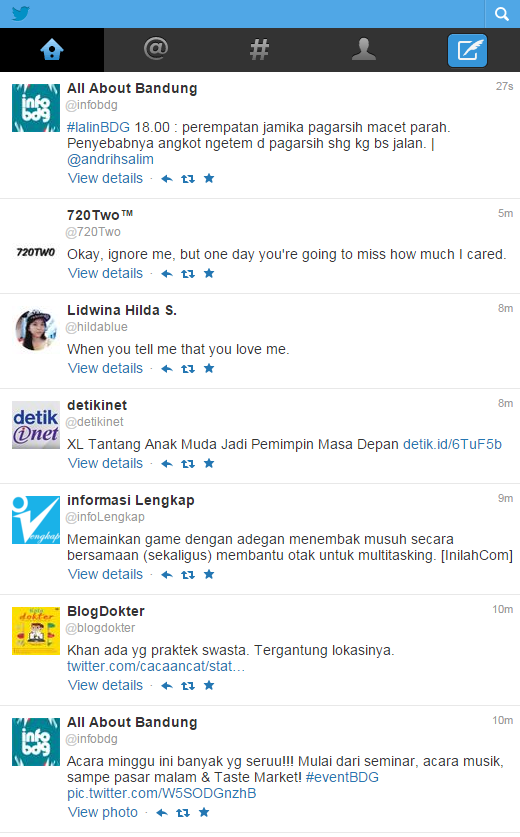
\includegraphics[width=1.00\textwidth]{C:/Skripsi/doc/DokumenSkripsi/Gambar/Homepage Mobile Twitter.PNG}
	\caption{Homepage Twitter versi mobile}
	\label{fig:Homepage Mobile Twitter}
\end{figure}


\begin{figure}[htbp]
	\centering
		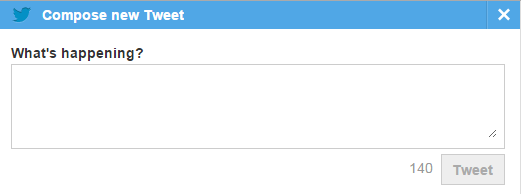
\includegraphics[width=1.00\textwidth]{C:/Skripsi/doc/DokumenSkripsi/Gambar/Textbox Mobile Tweet.PNG}
	\caption{Tampilan untuk melakukan tweet}
	\label{fig:Textbox Mobile Tweet}
\end{figure}

Setelah ada \textit{mention} yang ditujukan kepada Twitter Bot, aplikasi akan menangkap \textit{tweet} tersebut dan ditampilkan dalam bentuk pesan \textit{tweet} yang diterima oleh aplikasi. Hasil \textit{tweet} yang diterima aplikasi dapat dilihat pada gambar ~\ref{fig:HasilTangkapanTweetBerbasisTeks}. Setelah itu \textit{tweet} akan diperiksa oleh aplikasi apakah \textit{tweet} tersebut bertujuan untuk mencari jalur transportasi publik atau tidak. Jika benar, maka aplikasi akan melakukan proses pencarian jalur transportasi publik dan melakukan \textit{reply} atau balasan kepada pengguna. \textit{Reply tweet} tersebut berisikan jalur transportasi publik yang harus ditempuh kepada \textit{user}. Selain melakukan \textit{reply}, aplikasi juga menampilkan \textit{tweet} tersebut yang dapat dilihat pada gambar ~\ref{fig:HasilTweetBerbasisTeks}.

\begin{figure}
	\centering
		
\includegraphics{C:/Skripsi/doc/DokumenSkripsi/Gambar/HasilTangkapanTweetBerbasisTeks.PNG}
	\caption{Hasil streaming tweet}
	\label{fig:HasilTangkapanTweetBerbasisTeks}
\end{figure}

\begin{figure}
	\centering
		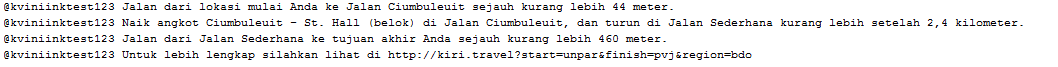
\includegraphics{C:/Skripsi/doc/DokumenSkripsi/Gambar/HasilTweetBerbasisTeks.PNG}
	\caption{Hasil balasan tweet kepada user}
	\label{fig:HasilTweetBerbasisTeks}
\end{figure}
\fi

\section{Pengujian}
Pada bagian ini akan dibahas mengenai hasil pengujian yang telah dilakukan terhadap aplikasi yang dibangun oleh penulis. Pengujian tersebut terdiri dari dua bagian, yaitu pengujian fungsional dan pengujian experimental. Pengujian fungsional bertujuan untuk memastikan semua fungsi aplikasi berjalan sesuai harapan. Sementara pengujian eksperimental bertujuan untuk mengetahui keberhasilan proses kerja dari aplikasi yang dibangun.

\subsection{Pengujian Fungsional}
Pengujian fungsional dilakukan pada fungsionalitas yang tersedia pada aplikasi yang dibangun. Pengujian ini dilakukan untuk mengetahui kesesuaian reaksi nyata dengan reaksi yang diharapkan dari aplikasi yang dibangun. Hasil pengujian ditunjukan pada tabel ~\ref{tab:TabelHasilPengujianFungsionalitasPadaAplikasiTwitterBotUntukMencariJalurTransportasiPublik}.

\begin{table}[h]
		\begin{tabular}{|p{0.5cm}|p{3cm}|p{5cm}|p{5cm}|}
			\hline
				No & Pengujian & Reaksi yang Diharapkan & Reaksi Aplikasi  \\ \hline
				1 & Melakukan otentikasi terhadap akun Twitter Bot & Otentikasi berhasil dilakukan antara Twitter dengan akun Twitter Bot. Otentikasi dilakukan dengan melakukan pemeriksaan terhadap \textit{ConsumerKey}, \textit{CustomerSecret}, \textit{AccessToken}, dan \textit{AccessTokenSecret} &  \textit{ConsumerKey}, \textit{CustomerSecret}, \textit{AccessToken}, dan \textit{AccessTokenSecret} yang diberikan Twitter berhasil diotentikasi oleh aplikasi \\ \hline
				2 & Melakukan \textit{streaming tweet} & Menangkap semua \textit{tweet} yang di\textit{mention} kepada akun @kviniink & Setiap \textit{tweet} yang di\textit{mention} kepada akun @kviniink dapat diterima secara \textit{realtime}\\ \hline
				3 & Membaca \textit{tweet} yang ditangkap & Melakukan pemeriksaan terhadap \textit{tweet} yang ditangkap, apakah \textit{tweet} tersebut merupakan \textit{tweet} untuk mencari transportasi publik atau bukan & Perangkat lunak dapat membedakan tweet untuk mencari jalur transportasi publik dengan tweet yang bukan bertujuan untuk mencari jalur transportasi publik  \\ \hline
				4 & Melakukan pencarian koordinat suatu lokasi menggunakan KIRI API & Mendapatkan hasil koordinat \textit{latitude} dan \textit{longitude} dari lokasi yang dicari & Perangkat lunak mendapatkan koordinat \textit{latitude} dan \textit{longitude} dari lokasi yang dicari  \\ \hline
				5 & Melakukan pencarian jalur transportasi publik menggunakan KIRI API & Mendapatkan jalur-jalur transportasi publik yang harus ditempuh dari lokasi awal menuju lokasi tujuan &  Perangkat lunak mendapatkan jalur-jalur transportasi publik yang harus ditempuh dari lokasi awal menuju lokasi tujuan \\ \hline
				6 & Melakukan tweet balasan & Membalas tweet dengan memberikan hasil pencarian jalur transportasi publik dengan format yang sudah ditentukan &  Akun @kviniink melakukan reply kepada akun penguji @kviniinktest123, reply tersebut berisikan jalur transportasi publik yang harus ditempuh dari lokasi awal menuju lokasi tujuan.\\ \hline
		\end{tabular}
	\caption{Tabel Hasil pengujian fungsionalitas pada Aplikasi Twitter Bot untuk mencari jalur transportasi publik}
	\label{tab:TabelHasilPengujianFungsionalitasPadaAplikasiTwitterBotUntukMencariJalurTransportasiPublik}
\end{table}

\iffalse
Pertama kali aplikasi dijalankan, aplikasi akan melakukan otentifikasi untuk melakukan Twitter \textit{stream} yang dapat dilihat pada gambar ~\ref{fig:StartingProgram}.

\begin{figure}[htbp]
	\centering
		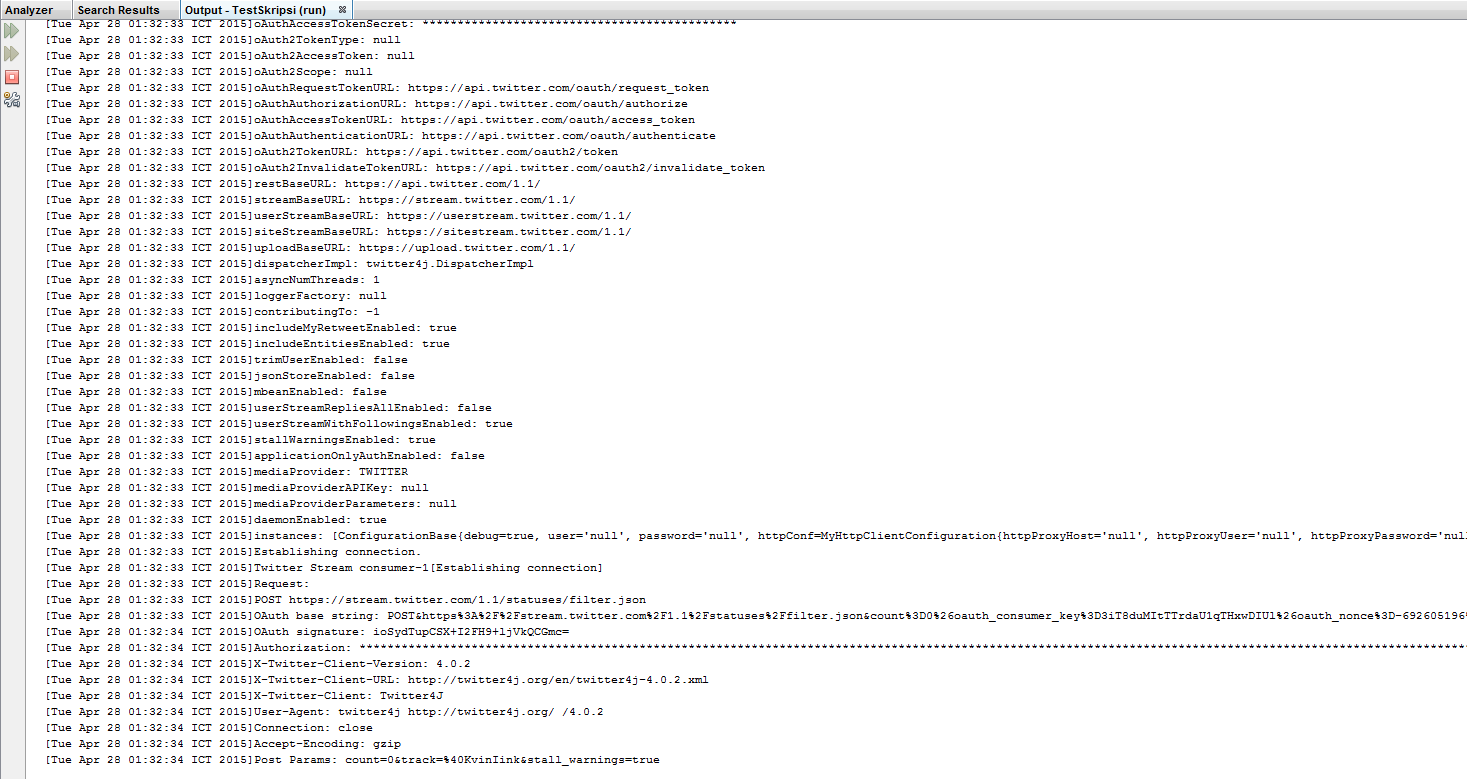
\includegraphics[width=1.00\textwidth]{C:/Skripsi/doc/DokumenSkripsi/Gambar/StartingProgram.PNG}
	\caption{Starting program}
	\label{fig:StartingProgram}
\end{figure}

Tweet dapat dilakukan dengan cara menuliskan pesan pada kotak yang sudah diset, disini user dapat menggunakannya untuk mencari jalur transportasi publik dengan cara melakukan \textit{mention} kepake @kiriupdate seperti yang ada di gambar ~\ref{fig:textboxTweet}.

\begin{figure}[htbp]
	\centering
		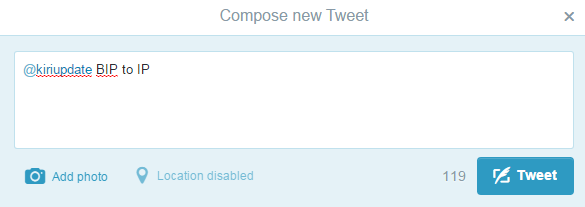
\includegraphics[width=1.00\textwidth]{C:/Skripsi/doc/DokumenSkripsi/Gambar/textboxTweet.PNG}
	\caption{Compose new Tweet}
	\label{fig:textboxTweet}
\end{figure}

Setelah melakukan \textit{tweet}, dapat dilihat pada gambar ~\ref{fig:SuccessTweetToKiriUpdate}. Maka program akan menangkap tweet tersebut, dapat dilihat pada gambar ~\ref{fig:TweetDitangkap}. Setelah itu tweet tersebut akan diolah untuk dicari rute transportasi publik tersebut. ??Apakah program harus memberi tampilan tentang bagaimana data diolah step by stepnya, dimulai dari mencari koordinat lokasi awal dan tujuan, sampai dengan hasil pencariannya??. Ketika selesai aplikasi akan membalas \textit{tweet} jalur transportasi publik kepada \textit{user} seperti yang ada di gambar ~\ref{fig:HasilTweet}.

\begin{figure}[htbp]
	\centering
		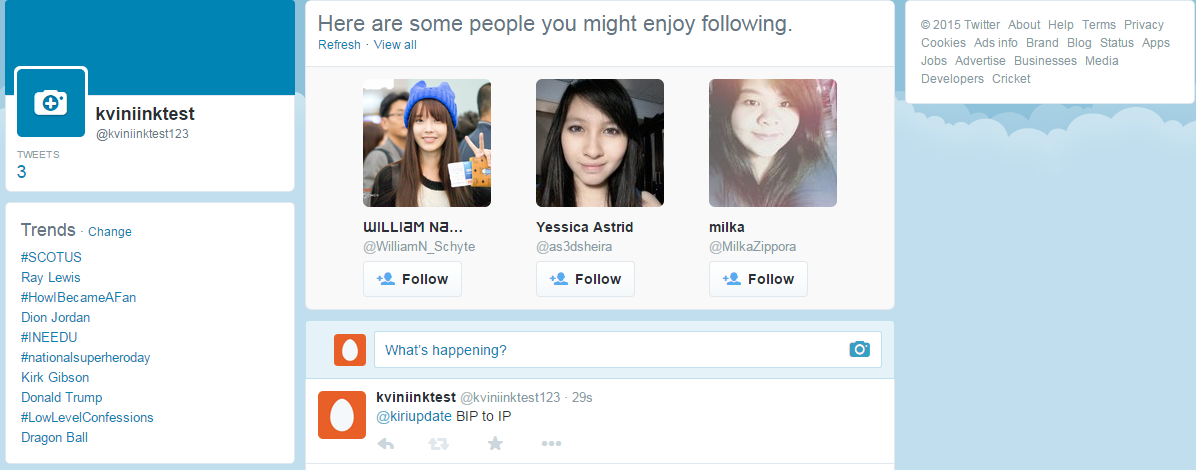
\includegraphics[width=1.00\textwidth]{C:/Skripsi/doc/DokumenSkripsi/Gambar/SuccessTweetToKiriUpdate.PNG}
	\caption{Tweet Kepada User @kiriupdate}
	\label{fig:SuccessTweetToKiriUpdate}
\end{figure}

\begin{figure}[htbp]
	\centering
		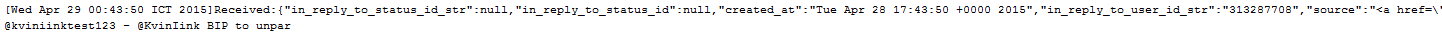
\includegraphics[width=1.00\textwidth]{C:/Skripsi/doc/DokumenSkripsi/Gambar/TweetDitangkap.PNG}
	\caption{Tweet Diterima oleh Aplikasi}
	\label{fig:TweetDitangkap}
\end{figure}

\begin{figure}[htbp]
	\centering
		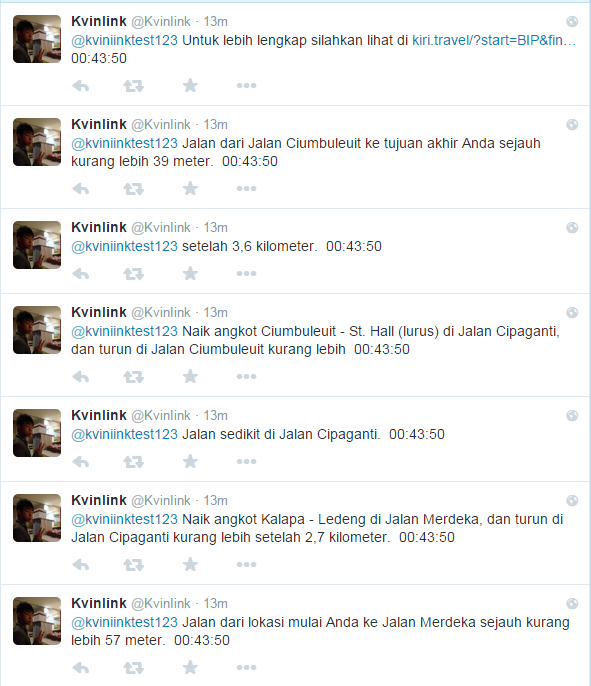
\includegraphics[width=1.00\textwidth]{C:/Skripsi/doc/DokumenSkripsi/Gambar/HasilTweet.PNG}
	\caption{Tweet Rute Jalur Transportasi Publik}
	\label{fig:HasilTweet}
\end{figure}
\fi
\subsection{Pengujian Eksperimental}
Pada sub bab ini akan dilakukan pengujian terhadap \textit{Twitter Bot} untuk mencari jalur transportasi publik. Peneliti meminta kepada beberapa orang untuk melakukan pencarian jalur transportasi publik kepada Twitter Bot untuk mencari jalur transportasi publik. Selain itu juga peneliti mencoba melakukan tweet pencarian melalui akun @kviniinktest123.

\begin{enumerate}
	\item Pengujian 1
	
	Pada pengujian 1, peneliti mencoba untuk mencari jalur transportasi publik untuk lokasi yang umum dikunjungi yaitu \textit{mall}. Pencarian dilakukan dengan lokasi awal adalah BIP (Bandung Indah Plaza) menuju lokasi tujuan adalah IP (Istana Plaza). Akun penguji @kviniinktest123 melakukan tweet kepada Twitter Bot akun @kviniink yang dapat dilihat pada gambar ~\ref{fig:Tweet1}.
	
	\begin{figure}
		\centering
			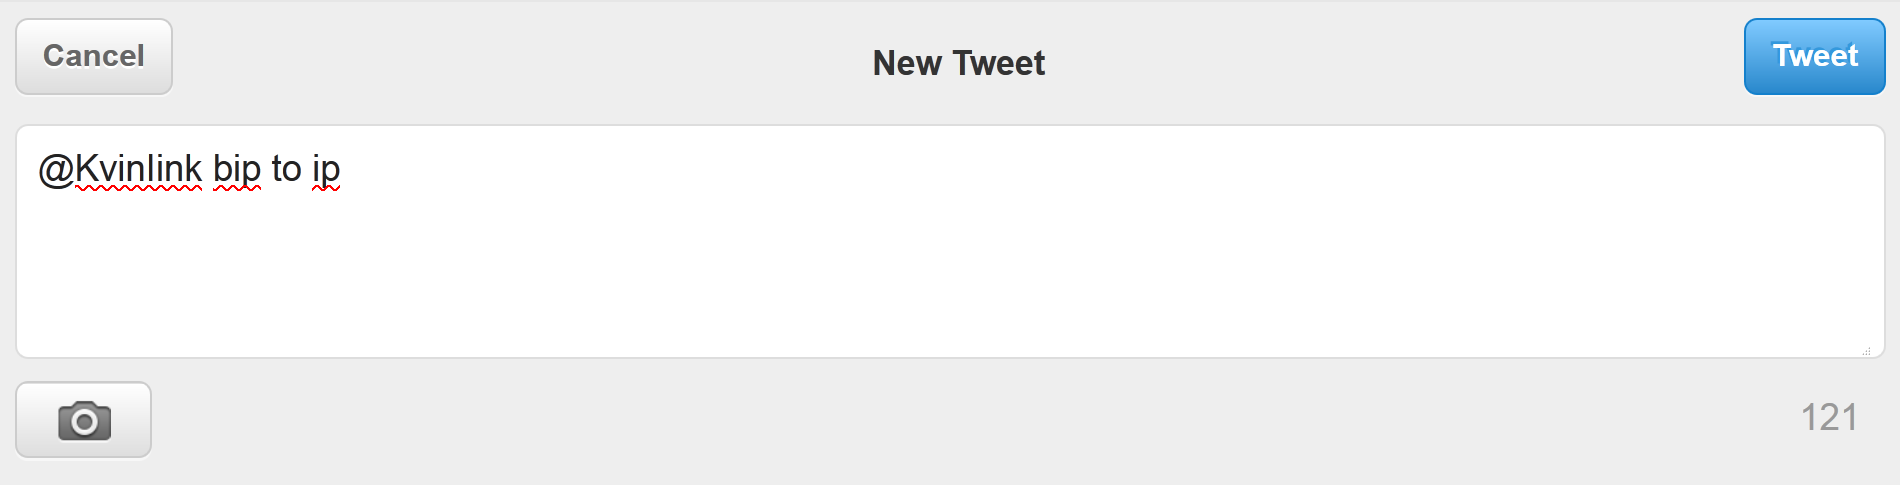
\includegraphics[width=0.75\textwidth]{C:/Skripsi/doc/DokumenSkripsi/Gambar/Tweet1.PNG}
		\caption{Tweet dari BIP menuju IP}
		\label{fig:Tweet1}
	\end{figure}
	
	Setelah proses \textit{tweet} dilakukan, Twitter Bot akan menangkap tweet tersebut dan memproses \textit{tweet}. Setelah proses pencarian selesai dilakukan, lalu Twitter Bot akun @kviniink melakukan \textit{reply} kepada akun @kviniinktest yang dapat dilihat pada gambar ~\ref{fig:HasilTweet1}. 
	
		
	\begin{figure}
		\centering
			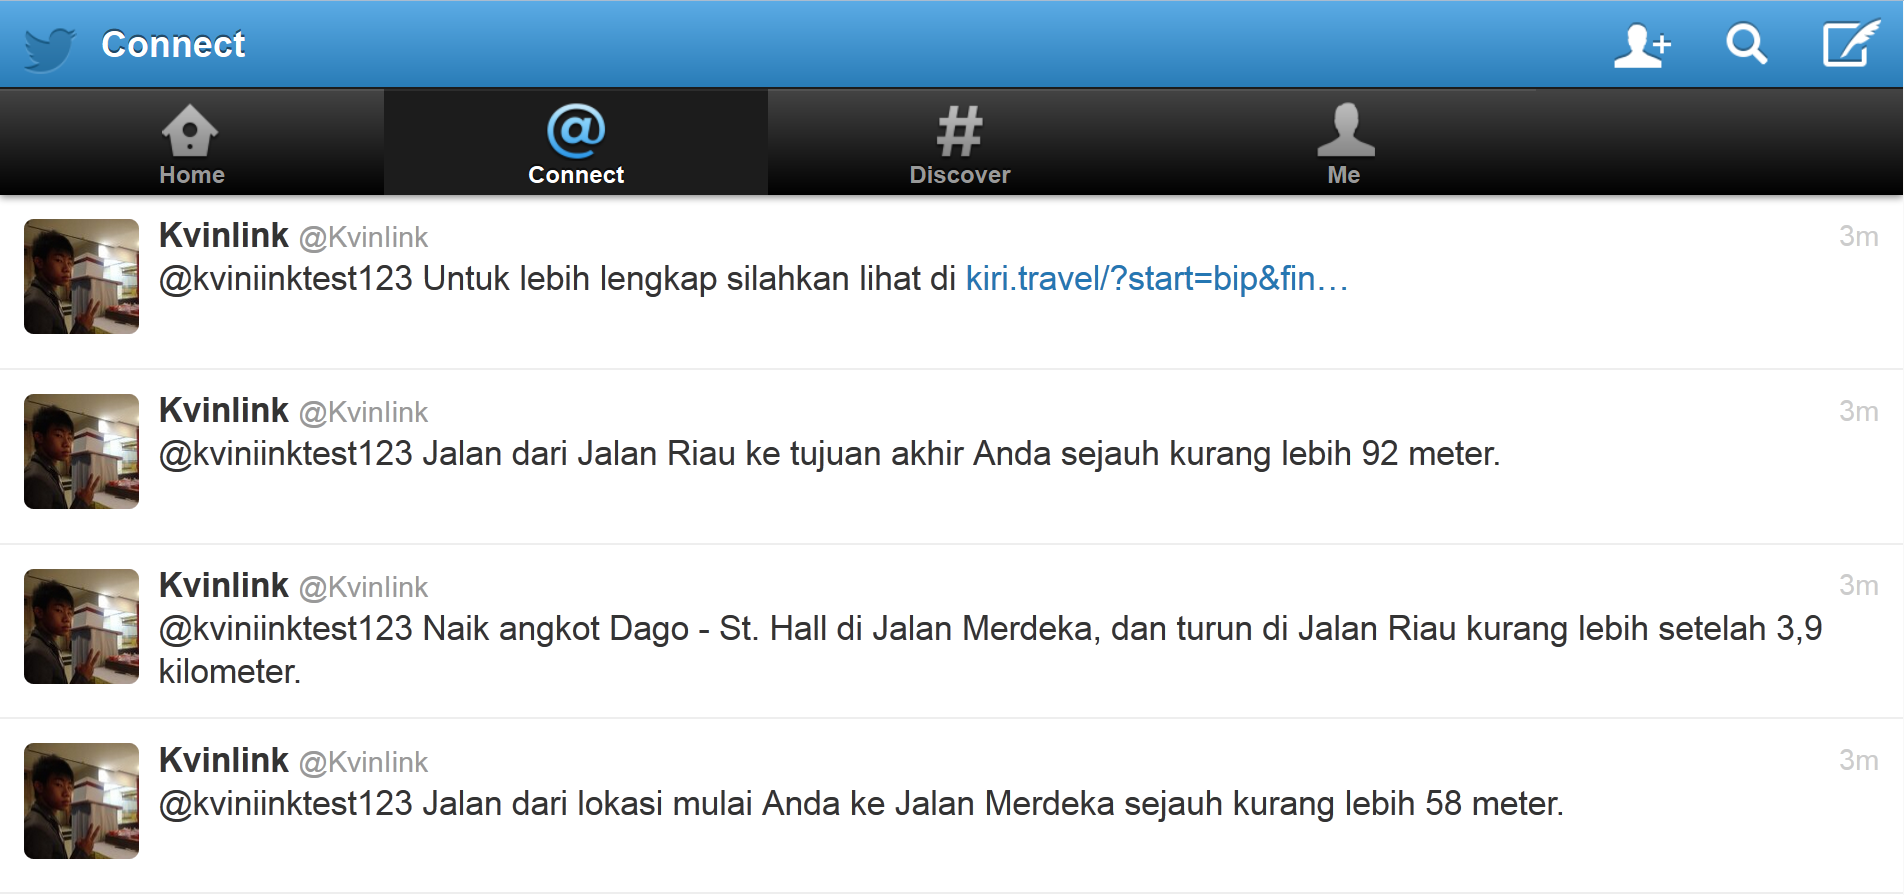
\includegraphics[width=0.75\textwidth]{C:/Skripsi/doc/DokumenSkripsi/Gambar/HasilTweet1.PNG}
		\caption{Hasil Pencarian Rute Transportasi Publik dari BIP menuju IP}
		\label{fig:HasilTweet1}
	\end{figure}
	
	Pencarian ke dua dilakukan pencarian dengan lokasi awal adalah BIP (Bandung Indah Plaza) dan lokasi tujuan ada PVJ (Paris van Java). Dapat dilihat pada gambar ~\ref{fig:Tweet2}, akun @kviniinktest123 melakukan \textit{tweet} pencarian jalur transportasi publik yang di \textit{mention} kepada akun @kviniink dengan lokasi awal adalah BIP dan lokasi tujuan adalah PVJ.
	
	\begin{figure}
		\centering
			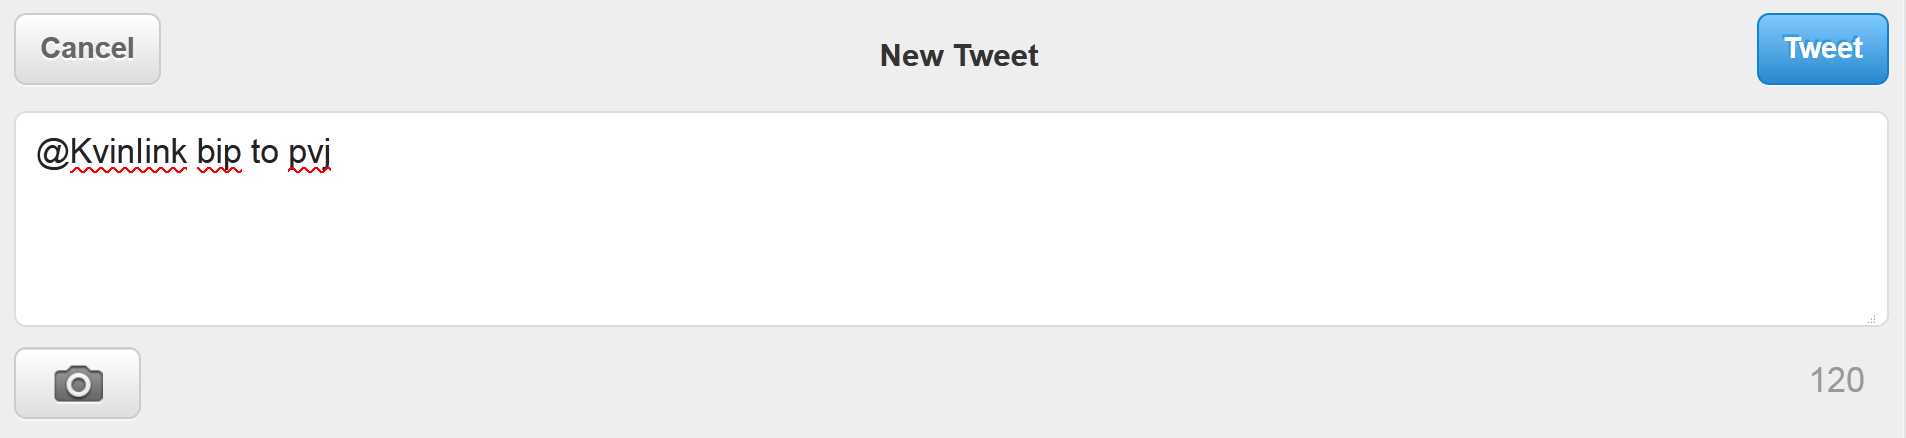
\includegraphics[width=0.75\textwidth]{C:/Skripsi/doc/DokumenSkripsi/Gambar/Tweet2.PNG}
		\caption{Tweet dari BIP menuju PVJ}
		\label{fig:Tweet2}
	\end{figure}
	
	Setelah itu tweet tersebut proses oleh aplikasi untuk dicari jalur transportasi publiknya, lalu Twitter Bot akun @kviniink melakukan \textit{reply} kepada akun @kviniinktest. Reply tweet tersebut merupakan jalur transportasi publik yang harus ditempuh, \textit{reply tweet} tersebut dapat dilihat pada gambar ~\ref{fig:HasilTweet2}.
	
	
	\begin{figure}
		\centering
			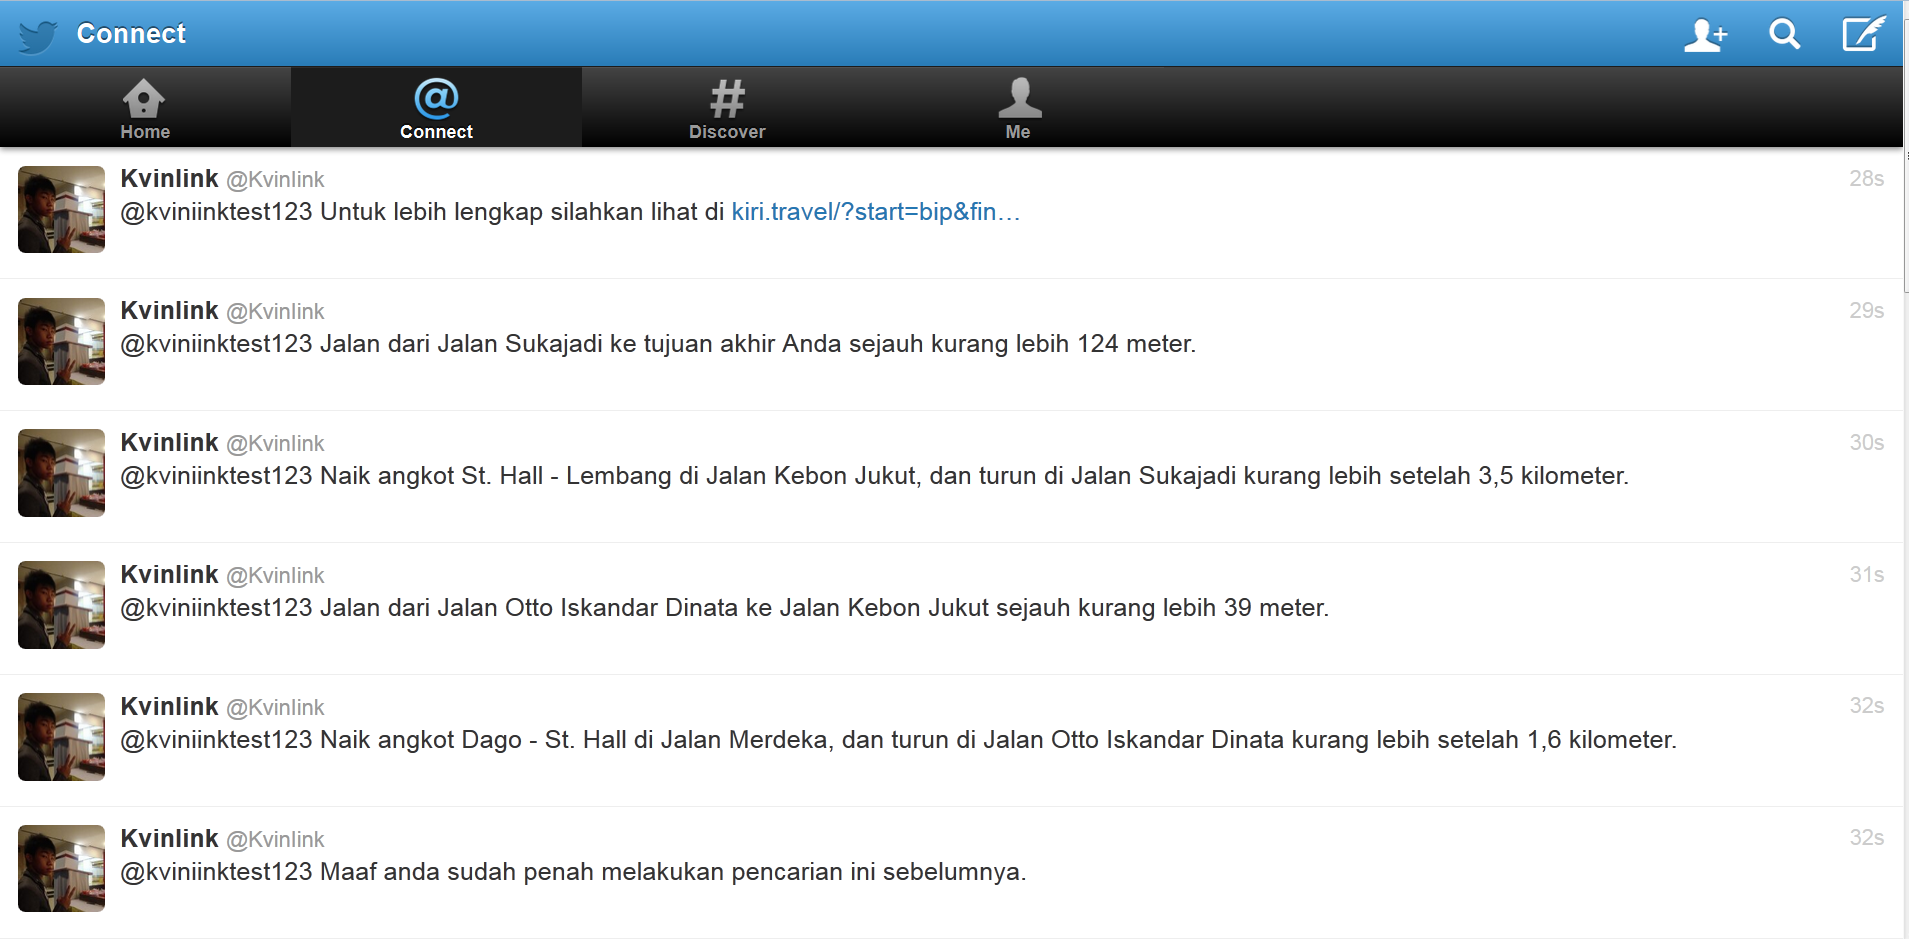
\includegraphics[width=0.75\textwidth]{C:/Skripsi/doc/DokumenSkripsi/Gambar/HasilTweet2.PNG}
		\caption{Hasil Pencarian Rute Transportasi Publik dari BIP menuju PVJ}
		\label{fig:HasilTweet2}
	\end{figure}
	
	Pada pencarian ke dua dapat dilihat pada tweet pertama terjadi ketidak sesuaian hasil dari KIRI API dengan hasil tweet.
	Peneliti lalu melakukan pencarian melalui website KIRI yaitu http://kiri.travel. Pencarian pertama dilakukan dengan lokasi awal adalah BIP dan lokasi tujuan adalah IP. Hasil pencarian KIRI tersebut dapat dilihat pada gambar ~\ref{fig:HasilKiri1}.
	
	
	\begin{figure}
		\centering
			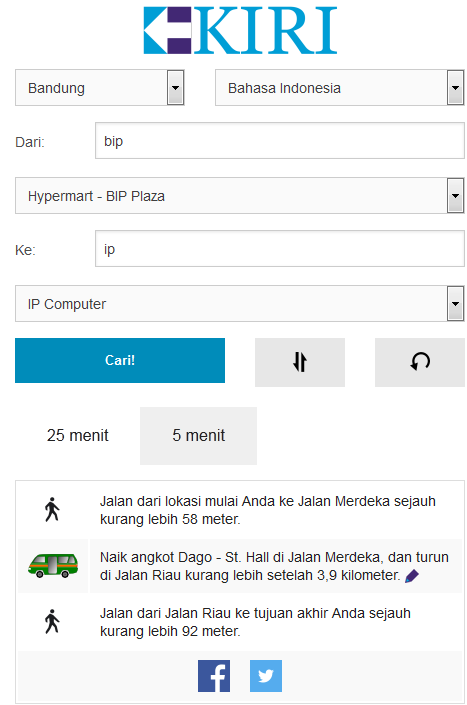
\includegraphics[width=0.75\textwidth]{C:/Skripsi/doc/DokumenSkripsi/Gambar/HasilKiri1.PNG}
		\caption{Hasil Pencarian Jalur Transportasi Publik dari BIP menuju IP Melalui Website KIRI}
		\label{fig:HasilKiri1}
	\end{figure}
	
	Lalu pencarian kedua dilakukan dengan lokasi awal adalah BIP dan lokasi tujuan adalah PVJ. Hasil pencarian KIRI dari BIP menuju PVJ dapat dilihat pada gambar ~\ref{fig:HasilKiri2}. Setelah dilihat dari hasil keduanya, Twitter Bot melakukan \textit{duplicate tweet} pada \textit{tweet} pertama pencarian ke dua. Untuk menghindari adanya duplicate tweet, peneliti menaruh waktu untuk jam, menit, dan detik di setiap tweet yang dilakukan oleh Twitter Bot agar membuat setiap tweet tersebut bersifat unik.
	
	\begin{figure}
		\centering
			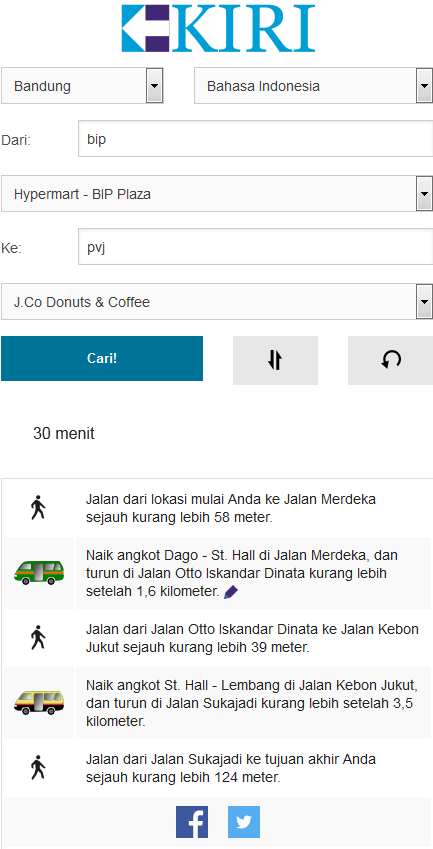
\includegraphics[width=0.75\textwidth]{C:/Skripsi/doc/DokumenSkripsi/Gambar/HasilKiri2.PNG}
		\caption{Hasil Pencarian Jalur Transportasi Publik dari BIP menuju PVJ Melalui Website KIRI}
		\label{fig:HasilKiri2}
	\end{figure}
	\clearpage
	
	\item Pengujian 2
	
	Pada pengujian 2, peneliti mencoba menjalankan aplikasi selama 24 jam dan meminta bantuan orang lain untuk melakukan \textit{tweet} pencarian jalur transportasi publik. Setelah ditambahkan waktu jam, menit, dan detik pada setiap \textit{tweet}, aplikasi \textit{Twitter bot} berjalan dengan lancar. \textit{Twitter bot} dapat memberitahu bahwa suatu lokasi pencarian tidak ditemukan yang dapat dilihat pada gambar ~\ref{fig:HasilFinal1}, akun @cla\_amour mencari lokasi tki dan kopo tetapi lokasi pencarian tidak ditemukan. Akun @cla\_amour juga mencari jalur transportasi publik yang lokasinya ditemukan tetapi tidak ada rute transportasi publiknya, hasil \textit{reply Twitter bot} dapat dilihat pada salah satu reply yang terdapat pada gambar ~\ref{fig:HasilFinal1}. Twitter bot tidak akan mendapatkan error ketika akun Twitter Bot @kviniink mendapat banyak mention dalam satu tweet seperti pada gambar ~\ref{fig:testTweet}, jika format penulisan benar maka Twitter bot akan tetap mencari jalur transportasi publiknya yang dapat dilihar pada gambar ~\ref{fig:hasilTestTweet}.
	
	
	\begin{figure}
		\centering
			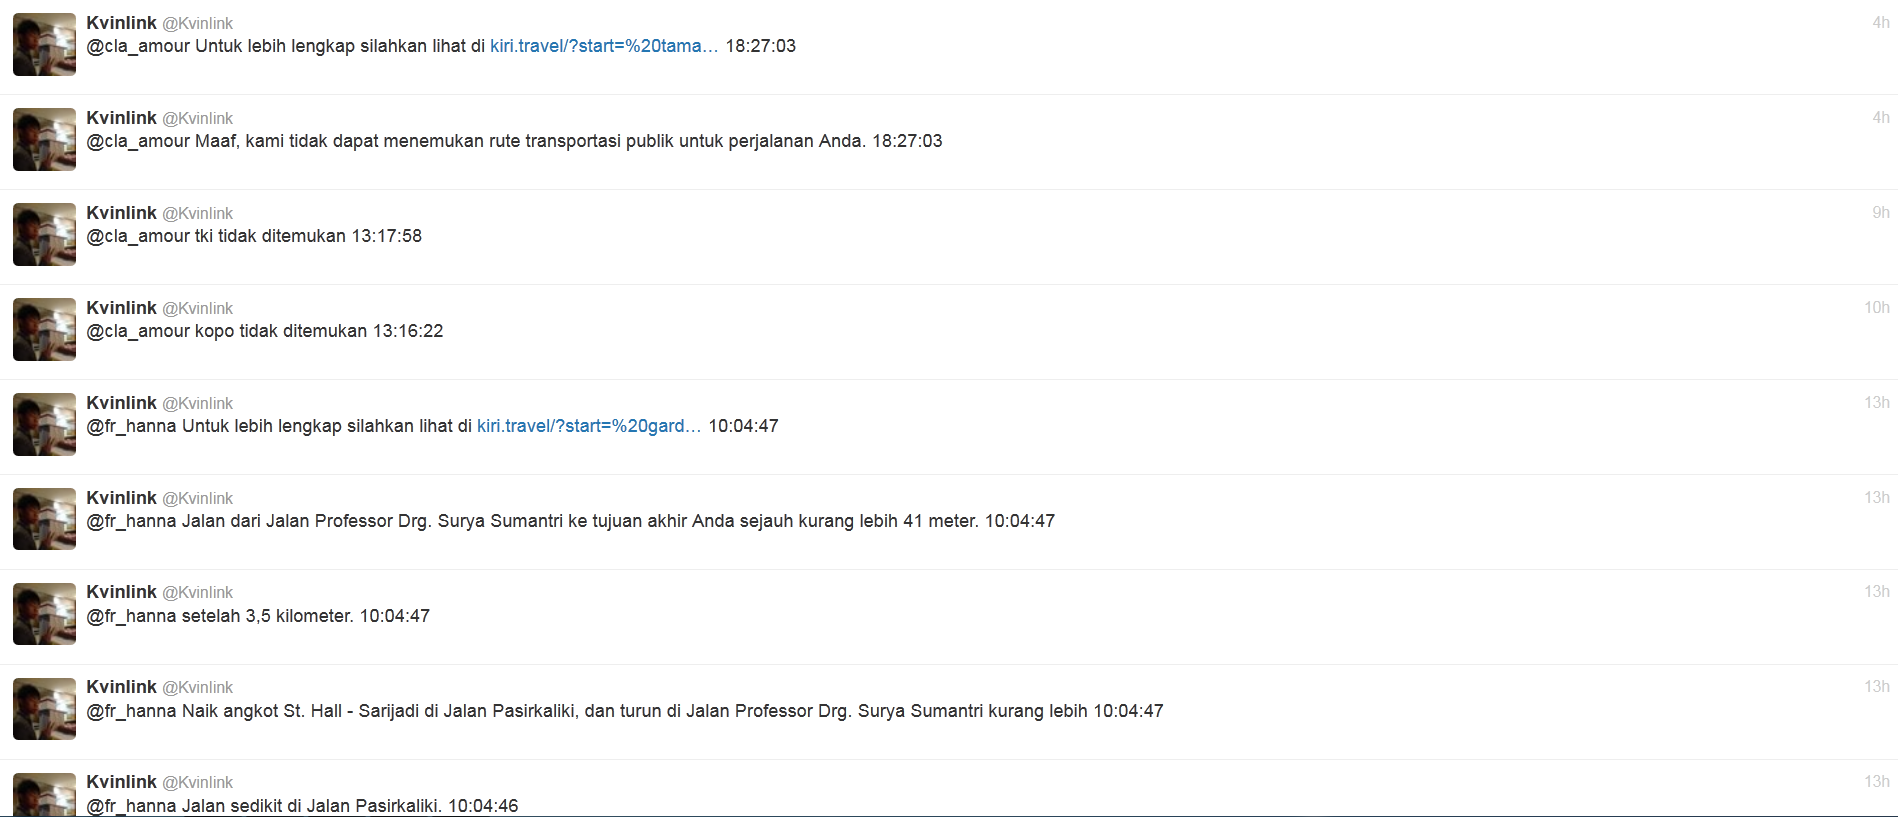
\includegraphics[width=0.9\textwidth]{C:/Skripsi/doc/DokumenSkripsi/Gambar/HasilFinal1.PNG}
		\caption{Hasil Reply Twitter Bot}
		\label{fig:HasilFinal1}
	\end{figure}
	
	\begin{figure}
		\centering
			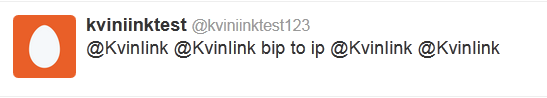
\includegraphics[width=0.9\textwidth]{C:/Skripsi/doc/DokumenSkripsi/Gambar/testTweet.PNG}
		\caption{Akun Twitter Bot Mendapat Banyak Mention Dalam Satu Tweet}
		\label{fig:testTweet}
	\end{figure}
	
	
	\begin{figure}
		\centering
			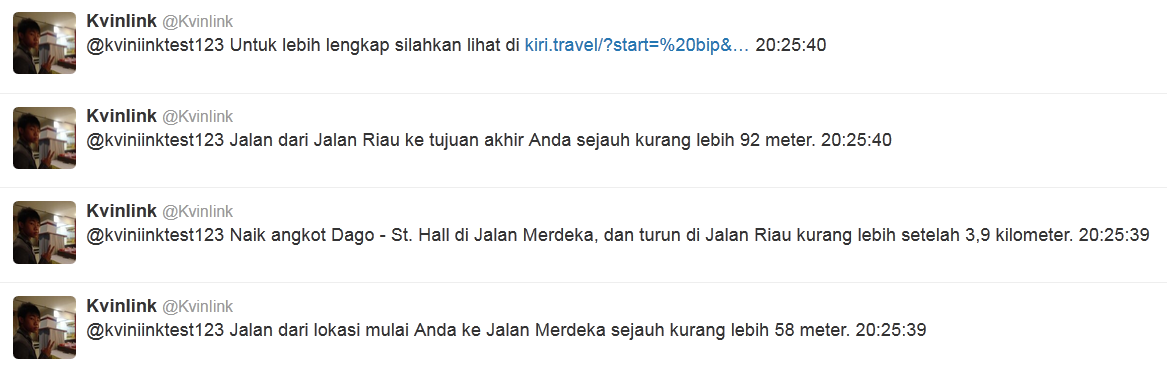
\includegraphics[width=0.9\textwidth]{C:/Skripsi/doc/DokumenSkripsi/Gambar/hasilTestTweet.PNG}
		\caption{Hasil Reply Twitter Bot}
		\label{fig:hasilTestTweet}
	\end{figure}

	Gambar ~\ref{fig:HasilFinal1} , gambar ~\ref{fig:HasilFinal2} , dan gambar ~\ref{fig:HasilFinal3} merupakan beberapa hasil reply dari Twitter Bot.
	
	
	\begin{figure}
		\centering
			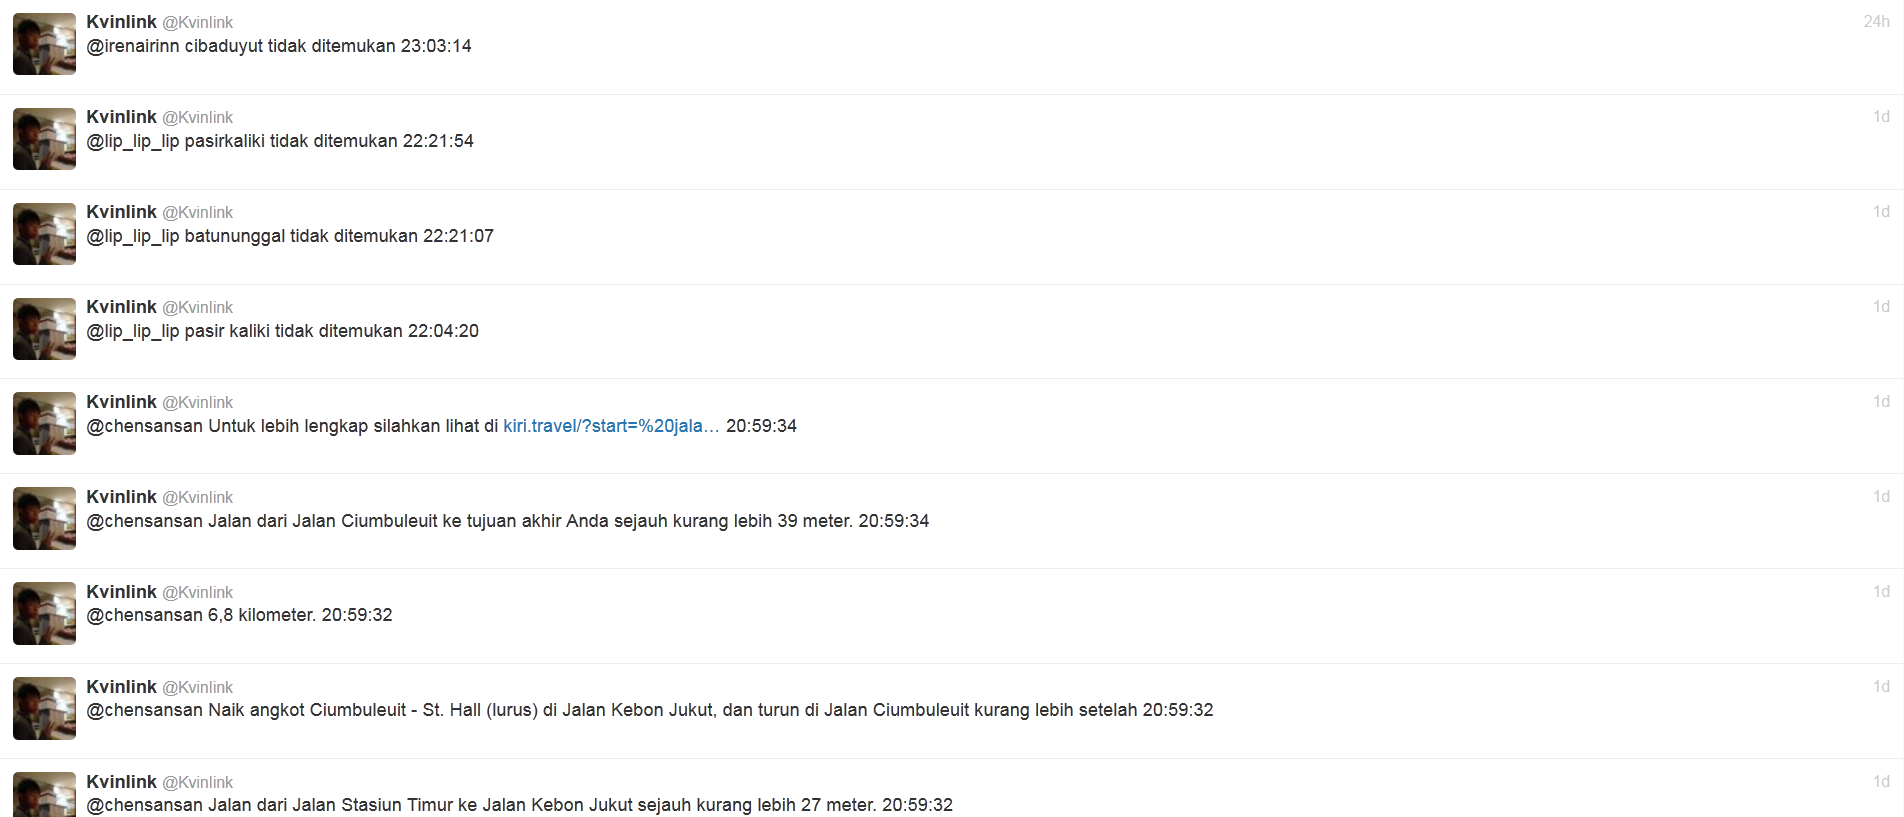
\includegraphics[width=0.9\textwidth]{C:/Skripsi/doc/DokumenSkripsi/Gambar/HasilFinal2.PNG}
			\caption{Hasil Reply Twitter Bot}
		\label{fig:HasilFinal2}
	\end{figure}
	
	\begin{figure}
		\centering
			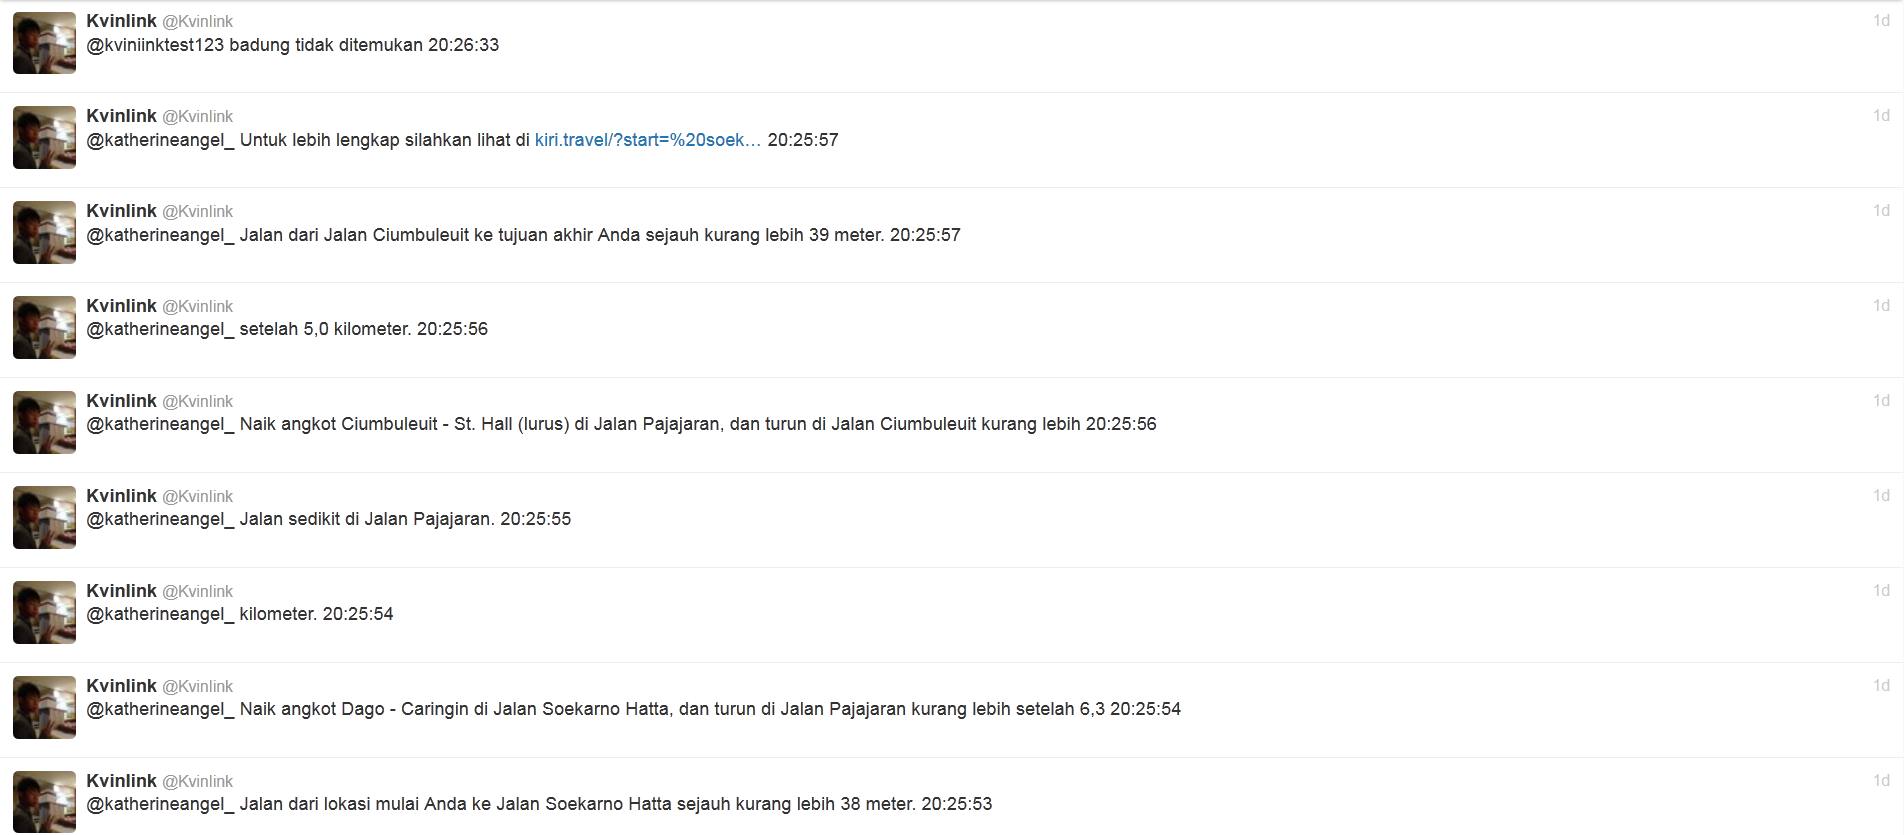
\includegraphics[width=0.9\textwidth]{C:/Skripsi/doc/DokumenSkripsi/Gambar/HasilFinal3.PNG}
			\caption{Hasil Reply Twitter Bot}
		\label{fig:HasilFinal3}
	\end{figure}
	
\end{enumerate}